\documentclass[]{article}
\usepackage{graphicx}
%\graphicspath{ {images/} }
\usepackage{wrapfig}
\usepackage{enumerate}
\usepackage{natbib}
\usepackage{url}
\usepackage{amsfonts}
\usepackage{mathtools}
\usepackage{subfig}

\newcommand{\ZZ}{\ensuremath{\mathbb{Z}}}
%opening
\title{CHVote: Efficient modular exponentiations}
\author{Nicolas GAILLY}

\begin{document}

\maketitle

\section{Introduction} \label{intro}

The canton of Geneva is working on a new digital votation system called
CHVote \cite{chvote} whose main goal is to increase the electorate confidence 
by providing a secure, transparent and usable online voting system. The final
product must enable a Swiss citizen to vote on any election mandated by the
Geneva canton using his laptop or mobile phone in a browser environment.

In this work, we focus on the vote casting part of the system from the client
side. In order to cast a vote, the client has to perform an k-out-of-n oblivious
transfer protocol \cite{chu2005} with the votation servers. In this protocol,
the client must perform between a few and a hundred of modular exponentiation
computation, depending on the number of votes the client has to perform for a
particular votation. In the context of CHVote, these modular exponentiation
computations take place in a multiplicative group whose order is a large prime
$q$. It is typically expected for security reason in this scenario that the number
of bits needed to represent q can lie between 1024 bits and up to 8192 bits.

The potentially large number of computation on the client side is problematic in
this context.  Indeed, modular exponentiation with a large modulo is a
computationally expensive operation. Typical optimization in this space has been
to provide hand written assembly code such as the GMP library \cite{gmplib}
coded in a mix of C and assembly. Unfortunately, such code is not able to run in
a browser environment. Therefore, the client typically has to rely on
Javascript, an interpreted language ran in the browser context to perform these
operations.  Unfortunately, Javascript performs quite poorly for such extensive
computations \cite{jsbad} and is therefore a poor executing environment for the
task.

In this work, we present an efficient way of computing these modular
exponentation relying on multiple third party servers. This work presents our
solution in section \ref{design}, our evaluation in section \ref{evaluation},
and finally some open questions to be addressed in section \ref{discussions}.

\section{Design} \label{design}

The goal of the project is to find an efficient scheme for the client to perform
modular exponentiations. In the context of CHVote, the client only must know
about the exponent; the base and the modulo need not to be private, simplifying
significantly the design of the solution.

The core idea is to decentralize the expensive computation to third party
servers while keeping the exponent secret by using a trivial non-threshold
secret sharing scheme. The client computes the final result from the individual
computations by using inexpensive modular \textit{multiplication}
operations.These servers are modeled as honest-but-curious adversaries and
should ideally be independent and highly available.


We assume we are working in a multiplicative group $G$ of order prime $q$. We denote
the base $b \in \ZZ_q^*$ and the exponent $a \in \ZZ_q^*$. We want to find an
efficient way to compute: $$ b^a \mod q $$

We call $S = \{s_1,\dots,s_n\}$ the set of $n$ servers selected to help
the client with his computation. The protocol works as follow:

\begin{enumerate}

    \item The client creates the $n$ shares:

        \begin{gather}
            \nonumber r_i = \text{\textit{ random }} \in \ZZ_q^* \text{  for } i=0...n-2\\
            \nonumber r_{n-1} = {a - \sum_{i=0}^{n-2} r_i} \mod q
        \end{gather}

    \item The client sends a computation request to each server $s_i$ over a
        secure channel. The request sent to server $i$ contains the share $r_i$,
        the base $b$ and the modulo $q$.
    \item Upon reception of a request, the server simply computes $ v_i = b^r_i
        \mod q$ and sends the response $v_i$ to the client.
    \item The client waits to receive $n$ responses and then computes the final
        result $v$ as: 

        \begin{align}
          \nonumber v &= \prod_{i=0}^{n-1} {v_i \mod q}\\
          \nonumber   &= b^{\sum_{i=0}^{n-1} r_i} \mod q\\
          \nonumber   &= b^{\sum_{i=0}^{n-2} r_i} * b^{r_{n-1}} \mod q\\
          \nonumber   &= b^a \mod q
        \end{align}

\end{enumerate}

This scheme allows an efficient outsourcing of the computation by allowing the
client to use only inexpensive operations.

\section{Evaluation} \label{evaluation}

In order to be relevant, this system must be able to outperform the performance
of the Javascript computation in a browser. In order to evaluate the system, we
have designed a Javascript benchmark framework enabling different strategies to be
evaluated. The code is available on Github \cite{code}.

The evaluation consists of comparing the time it takes to compute $N$ modular
exponentiations with Javascript and with the proposed system. The Javascript
code has been implemented using the JSBN library \cite{jsbn} which is the
fastest in the mathematical open source libraries in Javascript available. Only
three lines of code are needed to perform the computation using JSBN.  The
server side has been implemented as a web server using the Golang programming
language \cite{golang}. The web server listens for incoming HTTP POST requests
from the client containing the base, exponent and modulo.  The web server then
performs the computation using a binding to the GMP library \cite{gmplib} for
good performance and sends back the results. The format of the communication is
done through JSON with hexadecimal encoding of the parameters. 

The results can be found in the Figure~\ref{fig:system}. The proposed system clearly
outperforms Javascript by an order of magnitude for any number of requested
modular exponentations. Even for one modular exponentiation the system
outperforms JSBN by a factor of 3, although the simulation did not use any
secure connection that might add a constant to the overall time.

\begin{figure}[!htb]

    \centering

    \begin{center}
        \label{fig:system}
        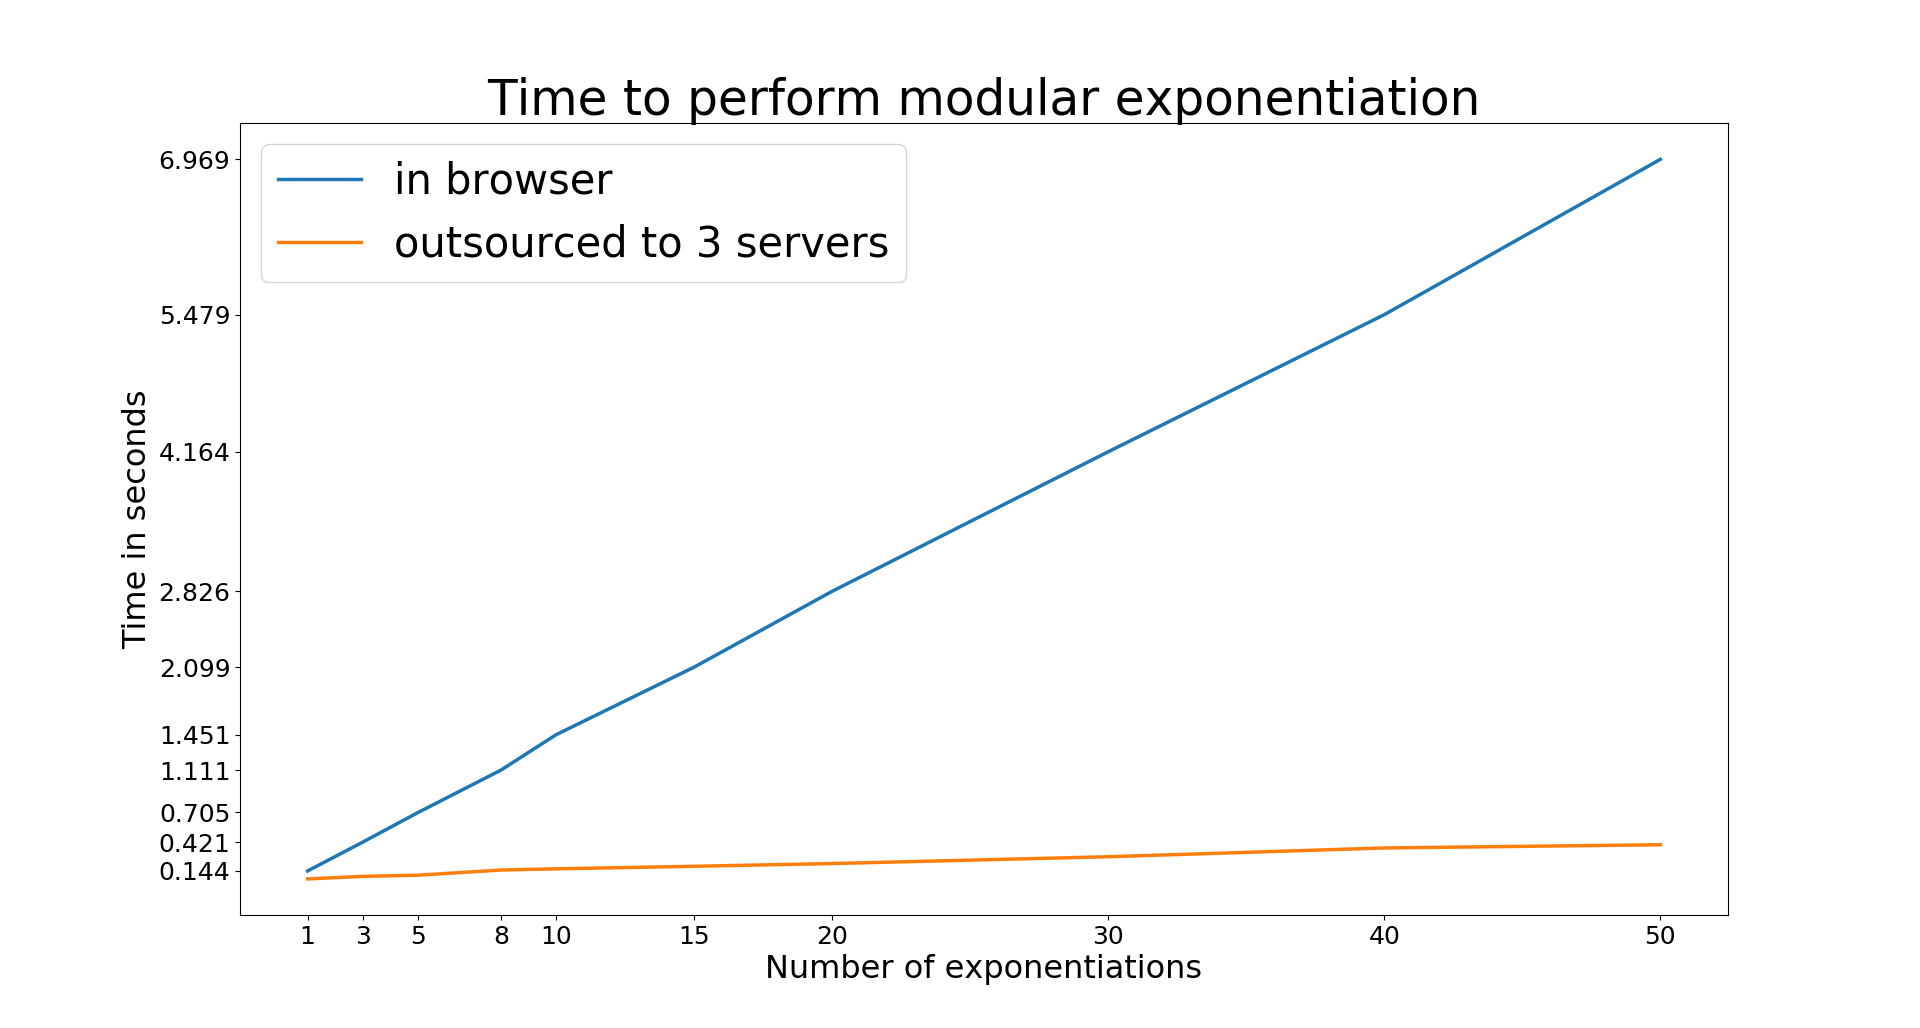
\includegraphics[scale=0.25]{local_vs_split_50.png}
        \caption{\textbf{Performance of the in-browser computation vs
        outsourced computation}.}
    \end{center}

\end{figure}

\section{Discussions} \label{discussions}

We discuss in this section some open questions and some hints for future work. 

\begin{enumerate} 
    \item One assumptions the system makes is that the server are
        honest-but-curious. If we want to relieve that assumption, the system
        needs a \textit{recovery} mechanism for the client to still be able to
        vote.  Some solutions may include the following: 
        \begin{itemize} 
            \item \textbf{Computing natively:} One solution can simply be to
                perform the computation using the native Javascript engine as a
                fallback mechanism. The client must be aware that the
                computation went wrong so he has an explicit reason to wait
                longer for the computation to finish.  
            \item \textbf{Invidividual verifiability:} Another solution can be
                to require each servers to provide a valid NIZK proof of
                exponentiation. In this case, this proof can be instantiated as
                a Schnorr signature using $r_i$ as the private key and $b^{r_i}$
                as the public key.  
        \end{itemize} 
    \item The current design only encompass one approach. New technologies such
        as WebAssembly \cite{wasm} enables compilation from C/C++ and Rust to a
        low level bytecode interpretable by the browser engine. WebAssembly
        might provide a browser-compatible version of the GMP library with good
        performance. However, WebAssembly is still in its early stage and there
        is only a limited support from vendors and browsers. Detecting if the
        browser can run WebAssembly could potentially open the way for a hybrid
        system.
\end{enumerate}

\section{Conclusion}

We presented a system decentralizing an expensive computation to lightweight
servers using the GMP computational library. The system shows a significant gain
in performance compared to a native Javascript implementation and is therefor,
a good target for the CHVote system.


\bibliographystyle{plain}
\bibliography{main}

\end{document}
